% Options for packages loaded elsewhere
\PassOptionsToPackage{unicode}{hyperref}
\PassOptionsToPackage{hyphens}{url}
\PassOptionsToPackage{dvipsnames,svgnames,x11names}{xcolor}
\documentclass[
  10pt,
]{article}
\usepackage{xcolor}
\usepackage[margin=2cm]{geometry}
\usepackage{amsmath,amssymb}
\setcounter{secnumdepth}{-\maxdimen} % remove section numbering
\usepackage{iftex}
\ifPDFTeX
  \usepackage[T1]{fontenc}
  \usepackage[utf8]{inputenc}
  \usepackage{textcomp} % provide euro and other symbols
\else % if luatex or xetex
  \usepackage{unicode-math} % this also loads fontspec
  \defaultfontfeatures{Scale=MatchLowercase}
  \defaultfontfeatures[\rmfamily]{Ligatures=TeX,Scale=1}
\fi
\usepackage{lmodern}
\ifPDFTeX\else
  % xetex/luatex font selection
  \setmainfont[]{Carlito}
  \setmonofont[]{Adwaita Mono}
\fi
% Use upquote if available, for straight quotes in verbatim environments
\IfFileExists{upquote.sty}{\usepackage{upquote}}{}
\IfFileExists{microtype.sty}{% use microtype if available
  \usepackage[]{microtype}
  \UseMicrotypeSet[protrusion]{basicmath} % disable protrusion for tt fonts
}{}
\makeatletter
\@ifundefined{KOMAClassName}{% if non-KOMA class
  \IfFileExists{parskip.sty}{%
    \usepackage{parskip}
  }{% else
    \setlength{\parindent}{0pt}
    \setlength{\parskip}{6pt plus 2pt minus 1pt}}
}{% if KOMA class
  \KOMAoptions{parskip=half}}
\makeatother
\usepackage{longtable,booktabs,array}
\usepackage{calc} % for calculating minipage widths
% Correct order of tables after \paragraph or \subparagraph
\usepackage{etoolbox}
\makeatletter
\patchcmd\longtable{\par}{\if@noskipsec\mbox{}\fi\par}{}{}
\makeatother
% Allow footnotes in longtable head/foot
\IfFileExists{footnotehyper.sty}{\usepackage{footnotehyper}}{\usepackage{footnote}}
\makesavenoteenv{longtable}
\usepackage{graphicx}
\makeatletter
\newsavebox\pandoc@box
\newcommand*\pandocbounded[1]{% scales image to fit in text height/width
  \sbox\pandoc@box{#1}%
  \Gscale@div\@tempa{\textheight}{\dimexpr\ht\pandoc@box+\dp\pandoc@box\relax}%
  \Gscale@div\@tempb{\linewidth}{\wd\pandoc@box}%
  \ifdim\@tempb\p@<\@tempa\p@\let\@tempa\@tempb\fi% select the smaller of both
  \ifdim\@tempa\p@<\p@\scalebox{\@tempa}{\usebox\pandoc@box}%
  \else\usebox{\pandoc@box}%
  \fi%
}
% Set default figure placement to htbp
\def\fps@figure{htbp}
\makeatother
\setlength{\emergencystretch}{3em} % prevent overfull lines
\providecommand{\tightlist}{%
  \setlength{\itemsep}{0pt}\setlength{\parskip}{0pt}}
% Shared LaTeX extras for the Kept report PDFs (scripts/reportlib.py)
\usepackage{etoolbox}
\AtBeginEnvironment{longtable}{\footnotesize}
\let\oldunderscore\_
\renewcommand{\_}{\oldunderscore\allowbreak}
\usepackage{xcolor}
\definecolor{keptred}{HTML}{C8102E}
\usepackage{titlesec}
\titleformat{\section}{\Large\bfseries\color{keptred}}{}{0em}{}
\titleformat{\subsection}{\large\bfseries}{}{0em}{}
\setlength{\parskip}{0.45em}
\setlength{\parindent}{0pt}
\renewcommand{\arraystretch}{1.15}
\usepackage{tikz}
\usetikzlibrary{positioning,arrows.meta,calc}
\definecolor{edge}{HTML}{7B8794}
\definecolor{kblue}{HTML}{2A78D6}
\definecolor{korange}{HTML}{E8833A}
\tikzset{
  step/.style={draw=edge, rounded corners=3pt, fill=white, align=center, font=\footnotesize, inner sep=4pt, text width=#1, minimum height=1.1cm},
  step/.default=2.6cm,
  hot/.style={draw=korange, line width=1.1pt},
  go/.style={-{Stealth[length=2mm]}, edge, line width=0.8pt},
}
\usepackage{bookmark}
\IfFileExists{xurl.sty}{\usepackage{xurl}}{} % add URL line breaks if available
\urlstyle{same}
\hypersetup{
  pdftitle={Data quality report},
  pdfauthor={Team Sharpe Shooters},
  colorlinks=true,
  linkcolor={keptred},
  filecolor={Maroon},
  citecolor={Blue},
  urlcolor={keptred},
  pdfcreator={LaTeX via pandoc}}

\title{Data quality report}
\usepackage{etoolbox}
\makeatletter
\providecommand{\subtitle}[1]{% add subtitle to \maketitle
  \apptocmd{\@title}{\par {\large #1 \par}}{}{}
}
\makeatother
\subtitle{Maple Bank collections release → Kept's golden C360 ·
deliverable 4}
\author{Team Sharpe Shooters}
\date{04 October 2026}

\begin{document}
\maketitle

{
\hypersetup{linkcolor=black}
\setcounter{tocdepth}{1}
\tableofcontents
}
\section{TL;DR}\label{tldr}

We took \textbf{31 tables / 68,162,322 records} of deliberately messy
bank data and turned them into one trusted record per person. Every
number here is a live query (\texttt{scripts/quality\_report\_full.py});
nothing's typed in.

\begin{longtable}[]{@{}
  >{\raggedright\arraybackslash}p{(\linewidth - 2\tabcolsep) * \real{0.5000}}
  >{\raggedright\arraybackslash}p{(\linewidth - 2\tabcolsep) * \real{0.5000}}@{}}
\toprule\noalign{}
\endhead
\bottomrule\noalign{}
\endlastfoot
Quality gate on the golden record & \textbf{PASS, all 8 rules} \\
Source keys → people & \textbf{3,840,513 → 1,052,300 golden IDs}
(biggest person: 12 keys) \\
Match precision, checked by a human & \textbf{99.3\%} (298/300; exact
140/140, Splink 158/160) \\
Kinds of data issue found and handled & \textbf{19} (worst: autopay /
pre-authorised-debit account at another bank (not one of our deposit
accounts), 64.70\% of its table) \\
Clusters we refused to auto-merge & 5,491 (two national IDs) + 7 (more
than 12 keys) \\
Training vs live feature values & PASS: 0 of 56,000 cells differ
(0.0000\%; the limit is 0.1\%). \\
PII left in 785,594 redacted notes and calls & \textbf{0} \\
\end{longtable}

\textbf{The vibe:} never guess. If a rule can't read a value, it goes
empty and into a quarantine table with the reason, instead of being
``fixed'' into something wrong. A wrong date of birth can merge two
strangers into one customer, and in collections that means calling the
wrong person about someone else's debt.

\section{1. How we checked}\label{how-we-checked}

\begin{center}
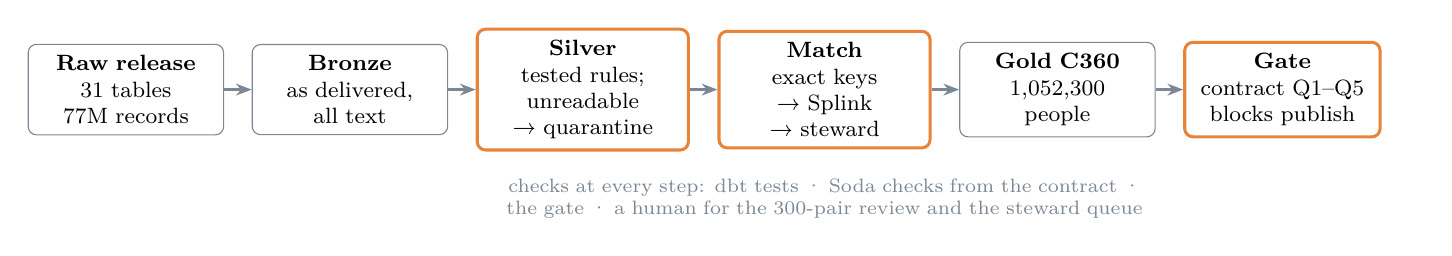
\begin{tikzpicture}[node distance=0.35cm]
\node[step=2.2cm] (raw) {\textbf{Raw release}\\ 31 tables\\ 77M records};
\node[step=2.2cm, right=of raw] (bronze) {\textbf{Bronze}\\ as delivered,\\ all text};
\node[step=2.4cm, right=of bronze, hot] (silver) {\textbf{Silver}\\ tested rules;\\ unreadable → quarantine};
\node[step=2.4cm, right=of silver, hot] (match) {\textbf{Match}\\ exact keys → Splink\\ → steward};
\node[step=2.2cm, right=of match] (gold) {\textbf{Gold C360}\\ 1,052,300\\ people};
\node[step=2.2cm, right=of gold, hot] (gate) {\textbf{Gate}\\ contract Q1–Q5\\ blocks publish};
\foreach \a/\b in {raw/bronze, bronze/silver, silver/match, match/gold, gold/gate} \draw[go] (\a) -- (\b);
\node[font=\scriptsize, text=edge, below=0.25cm of match, text width=15cm, align=center]
  {checks at every step: dbt tests · Soda checks from the contract · the gate · a human for the 300-pair review and the steward queue};
\end{tikzpicture}
\end{center}

\begin{itemize}
\tightlist
\item
  \textbf{Land raw, clean after.} Bronze keeps every file exactly as it
  came, all columns as text, so nothing gets silently converted (the
  README warns \texttt{NA} is a real outcome code and IDs have leading
  zeros; both survive).
\item
  \textbf{Small tested rules} in \texttt{kept.data.clean} /
  \texttt{kept.data.traps} do the cleaning: names, dates, phones, postal
  codes, provinces, snapshots, the renamed column.
\item
  \textbf{Four layers of checks:} dbt tests on every model (gold types
  enforced), Soda checks generated from the data contract, the contract
  gate (\texttt{kept\ gate}, blocks publishing), and a human for what
  code can't decide (300 sampled matches, the steward queue).
\end{itemize}

\section{2. What's in the release}\label{whats-in-the-release}

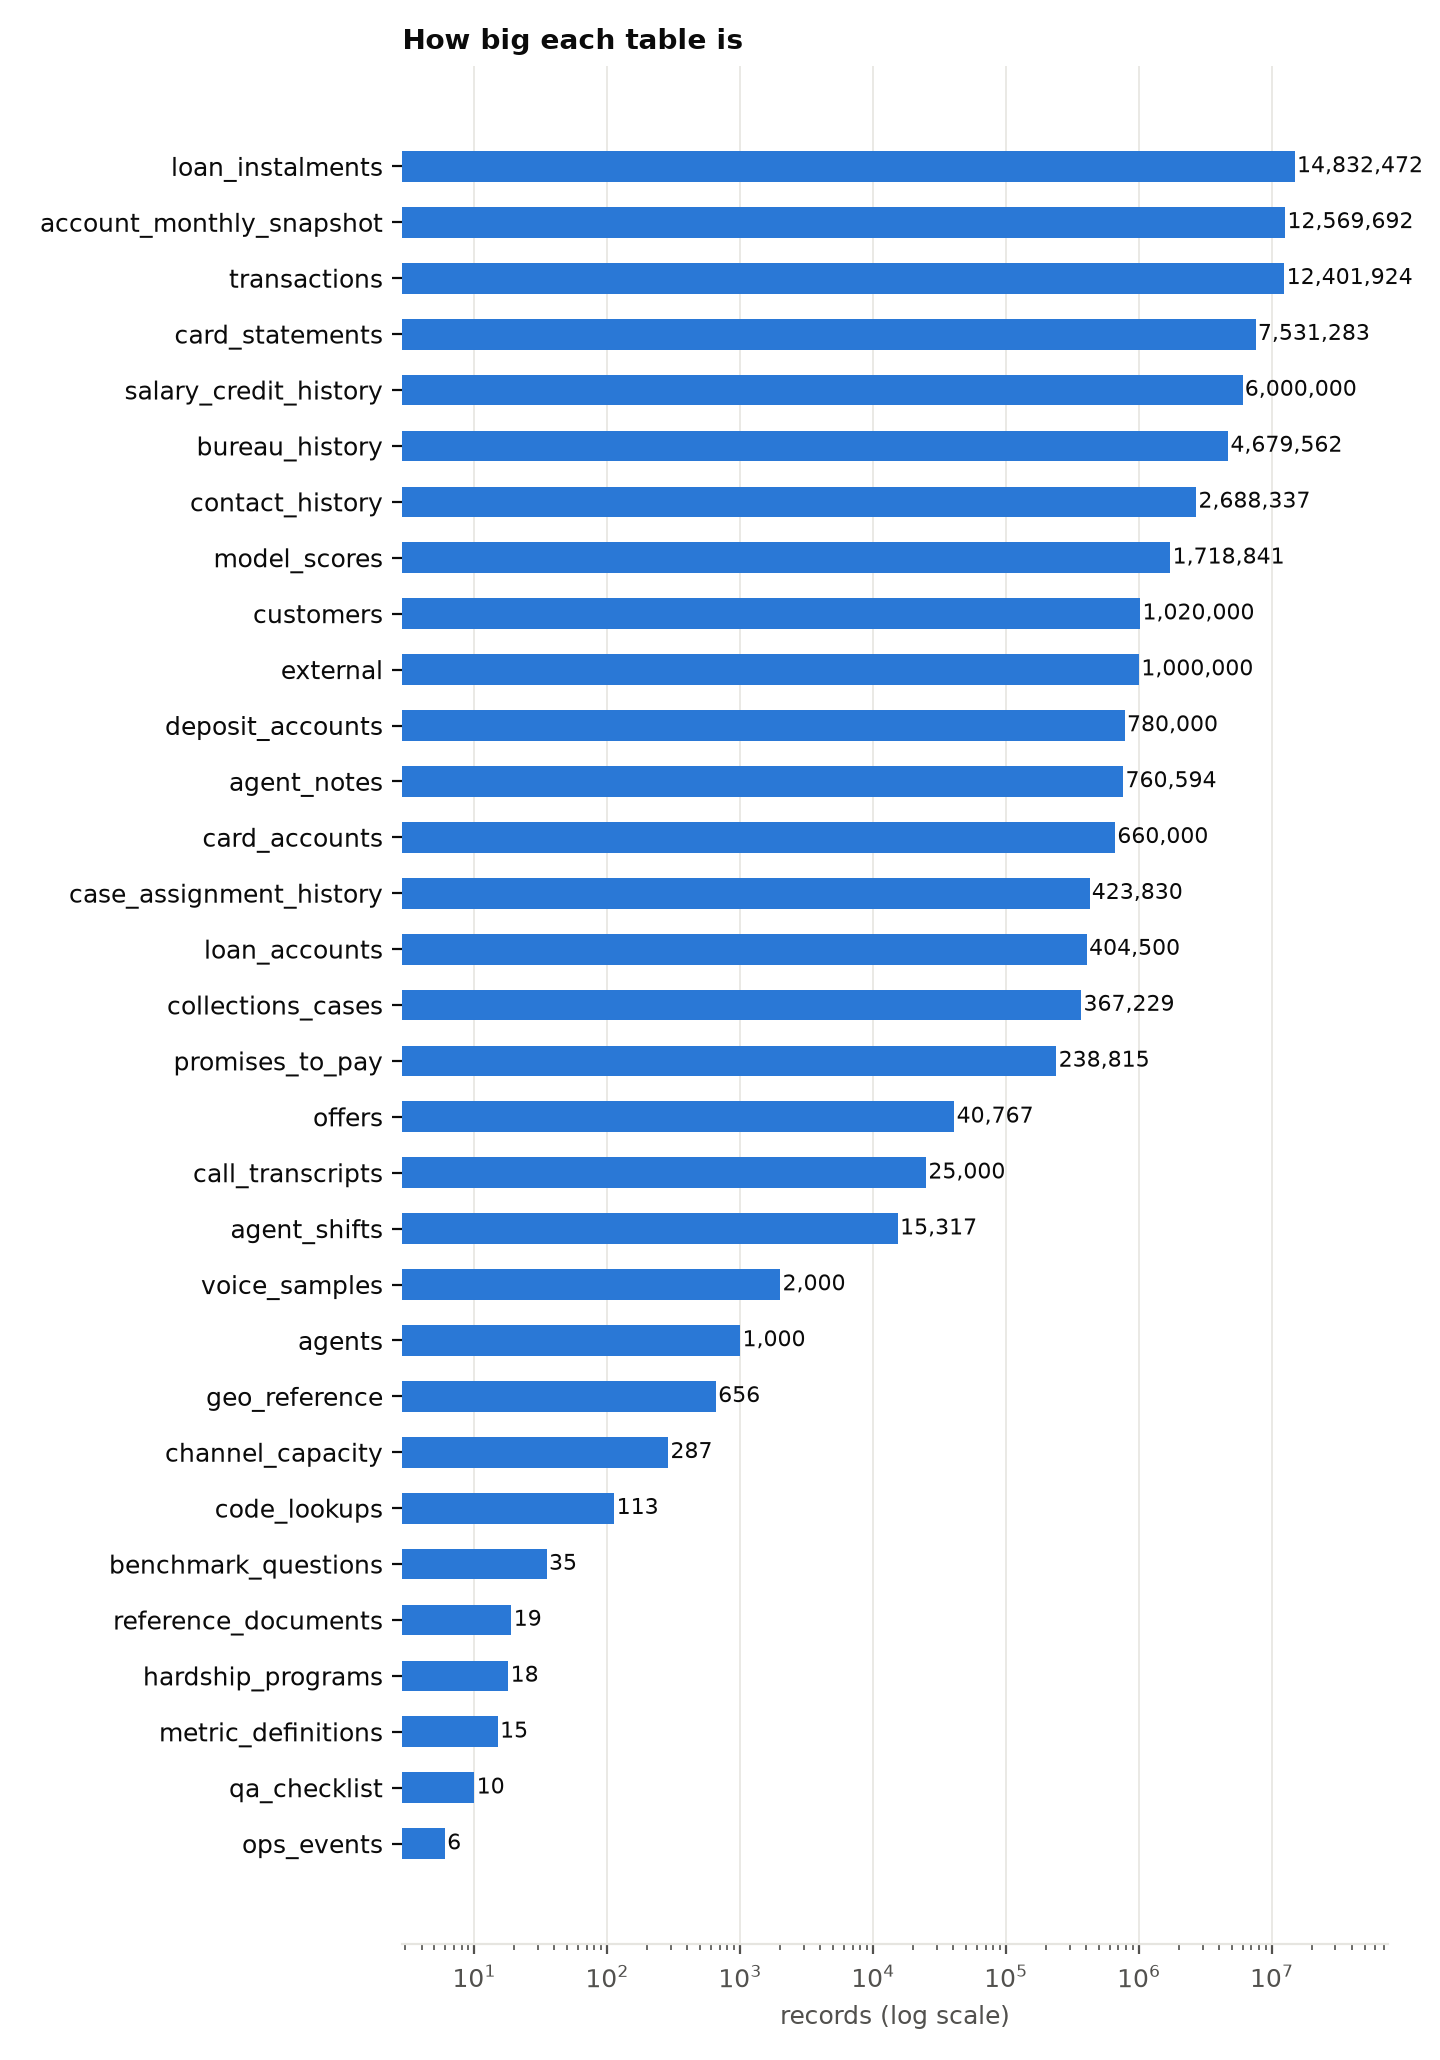
\includegraphics[width=1\linewidth,height=\textheight,keepaspectratio]{docs/reports/figures/q_rows.png}

Missing values are mostly by design: a charge-off date only exists if
the account was charged off, a reversal ID only if the transaction was
reversed. So high numbers here aren't bugs; §3 is where the real
problems are.

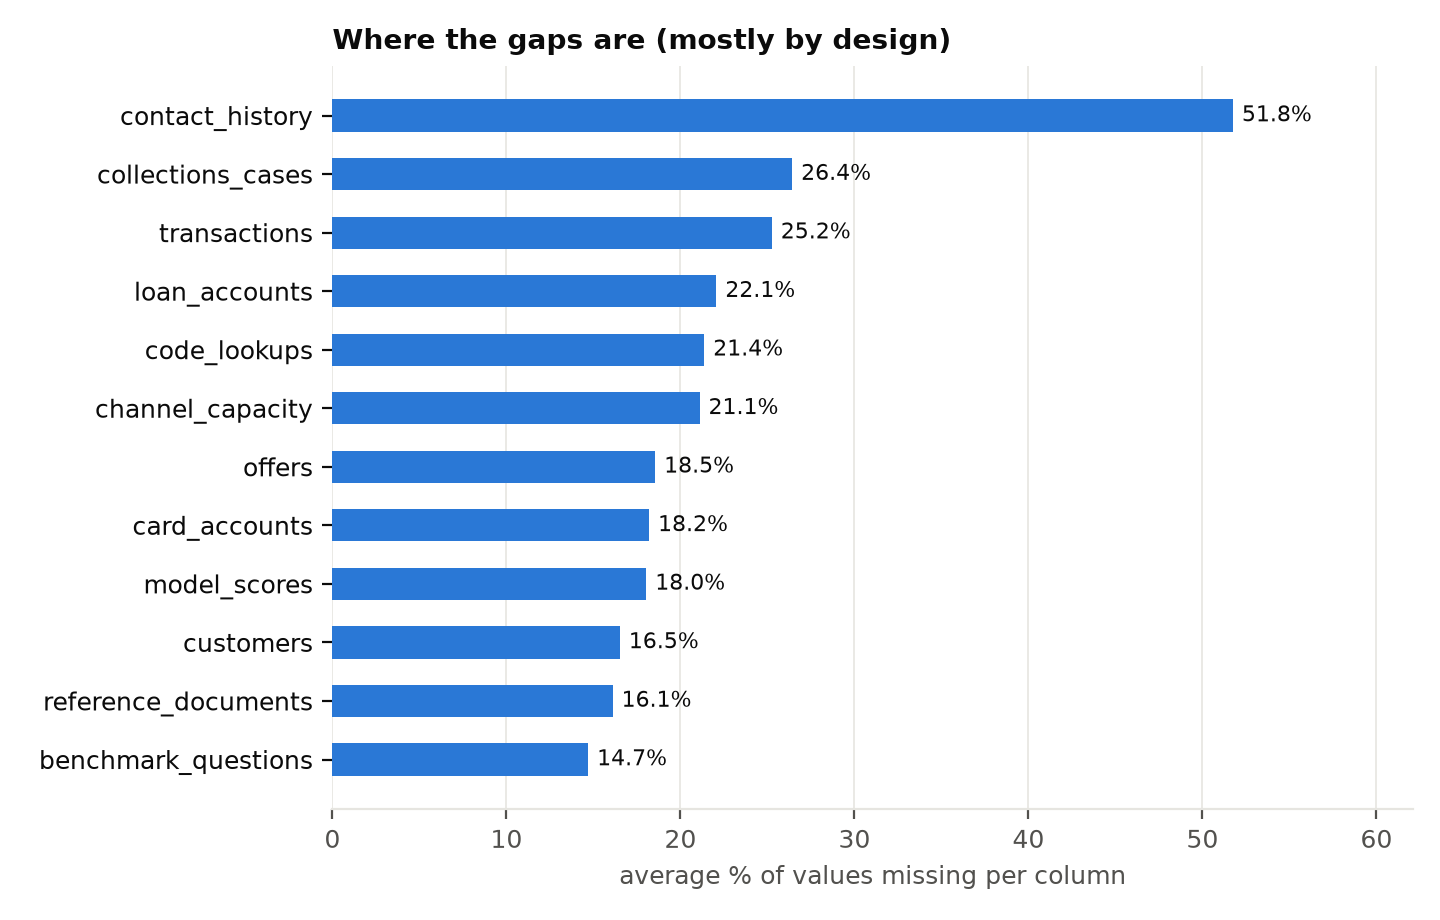
\includegraphics[width=1\linewidth,height=\textheight,keepaspectratio]{docs/reports/figures/q_nulls.png}

\begin{longtable}[]{@{}
  >{\raggedright\arraybackslash}p{(\linewidth - 10\tabcolsep) * \real{0.1667}}
  >{\raggedleft\arraybackslash}p{(\linewidth - 10\tabcolsep) * \real{0.1667}}
  >{\raggedleft\arraybackslash}p{(\linewidth - 10\tabcolsep) * \real{0.1667}}
  >{\raggedleft\arraybackslash}p{(\linewidth - 10\tabcolsep) * \real{0.1667}}
  >{\raggedleft\arraybackslash}p{(\linewidth - 10\tabcolsep) * \real{0.1667}}
  >{\raggedright\arraybackslash}p{(\linewidth - 10\tabcolsep) * \real{0.1667}}@{}}
\toprule\noalign{}
\begin{minipage}[b]{\linewidth}\raggedright
Table
\end{minipage} & \begin{minipage}[b]{\linewidth}\raggedleft
Rows
\end{minipage} & \begin{minipage}[b]{\linewidth}\raggedleft
Cols
\end{minipage} & \begin{minipage}[b]{\linewidth}\raggedleft
Cols with gaps
\end{minipage} & \begin{minipage}[b]{\linewidth}\raggedleft
Avg \% missing
\end{minipage} & \begin{minipage}[b]{\linewidth}\raggedright
Emptiest columns
\end{minipage} \\
\midrule\noalign{}
\endhead
\bottomrule\noalign{}
\endlastfoot
\texttt{loan\_instalments} & 14,832,472 & 19 & 5 & 13.5 &
\texttt{days\_late\_when\_paid}, \texttt{pad\_retry\_date} \\
\texttt{account\_monthly\_snapshot} & 12,569,692 & 16 & 5 & 13.1 &
\texttt{salary\_credit\_amount}, \texttt{limit\_or\_original\_amount} \\
\texttt{transactions} & 12,401,924 & 25 & 10 & 25.2 &
\texttt{reversal\_of\_txn\_id}, \texttt{return\_reason} \\
\texttt{card\_statements} & 7,531,283 & 26 & 3 & 7.8 &
\texttt{days\_late}, \texttt{first\_payment\_after\_due\_date} \\
\texttt{salary\_credit\_history} & 6,000,000 & 11 & 2 & 5.5 &
\texttt{first\_credit\_date}, \texttt{last\_credit\_date} \\
\texttt{bureau\_history} & 4,679,562 & 10 & 1 & 0.5 &
\texttt{risk\_score} \\
\texttt{contact\_history} & 2,688,337 & 128 & 90 & 51.8 &
\texttt{record\_hash}, \texttt{voice\_sample\_id} \\
\texttt{model\_scores} & 1,718,841 & 33 & 15 & 18.0 &
\texttt{predicted\_value}, \texttt{ptp\_id} \\
\texttt{customers} & 1,020,000 & 148 & 66 & 16.5 &
\texttt{record\_hash}, \texttt{duplicate\_of\_crm\_id} \\
\texttt{external} & 1,000,000 & 122 & 32 & 10.3 &
\texttt{public\_record\_date}, \texttt{risk\_score\_m01} \\
\texttt{deposit\_accounts} & 780,000 & 145 & 19 & 8.3 &
\texttt{freeze\_reason}, \texttt{overdraft\_dpd} \\
\texttt{agent\_notes} & 760,594 & 26 & 6 & 8.9 &
\texttt{last\_edited\_ts}, \texttt{template\_id} \\
\texttt{card\_accounts} & 660,000 & 148 & 75 & 18.2 &
\texttt{chargeoff\_date}, \texttt{chargeoff\_amount} \\
\texttt{case\_assignment\_history} & 423,830 & 23 & 2 & 2.0 &
\texttt{routing\_rule\_id}, \texttt{unassigned\_ts} \\
\texttt{loan\_accounts} & 404,500 & 135 & 76 & 22.1 &
\texttt{chargeoff\_date}, \texttt{chargeoff\_amount} \\
\texttt{collections\_cases} & 367,229 & 132 & 59 & 26.4 &
\texttt{record\_hash}, \texttt{agency\_name} \\
\texttt{promises\_to\_pay} & 238,815 & 29 & 7 & 8.0 &
\texttt{broken\_reason\_agent\_coded}, \texttt{paid\_date} \\
\texttt{offers} & 40,767 & 19 & 8 & 18.5 & \texttt{decline\_reason},
\texttt{plan\_start\_date} \\
\texttt{call\_transcripts} & 25,000 & 29 & 1 & 3.2 &
\texttt{voice\_sample\_id} \\
\texttt{agent\_shifts} & 15,317 & 15 & 2 & 9.5 &
\texttt{absence\_reason}, \texttt{worked\_minutes} \\
\texttt{voice\_samples} & 2,000 & 34 & 1 & 0.9 &
\texttt{channel\_map} \\
\texttt{agents} & 1,000 & 30 & 0 & 0.0 & -- \\
\texttt{geo\_reference} & 656 & 15 & 1 & 1.0 & \texttt{cma\_name} \\
\texttt{channel\_capacity} & 287 & 11 & 4 & 21.1 &
\texttt{ops\_event\_id}, \texttt{daily\_budget\_cad} \\
\texttt{code\_lookups} & 113 & 7 & 2 & 21.4 & \texttt{description\_fr},
\texttt{attributes\_json} \\
\texttt{benchmark\_questions} & 35 & 7 & 2 & 14.7 & \texttt{metric\_id},
\texttt{tolerance} \\
\texttt{reference\_documents} & 19 & 17 & 3 & 16.1 &
\texttt{related\_table}, \texttt{superseded\_by} \\
\texttt{hardship\_programs} & 18 & 21 & 3 & 8.5 &
\texttt{term\_extension\_max\_months}, \texttt{rate\_override} \\
\texttt{metric\_definitions} & 15 & 14 & 0 & 0.0 & -- \\
\texttt{qa\_checklist} & 10 & 10 & 0 & 0.0 & -- \\
\texttt{ops\_events} & 6 & 10 & 1 & 3.3 & \texttt{reference\_doc\_id} \\
\end{longtable}

\section{3. The issues, and what we did about
each}\label{the-issues-and-what-we-did-about-each}

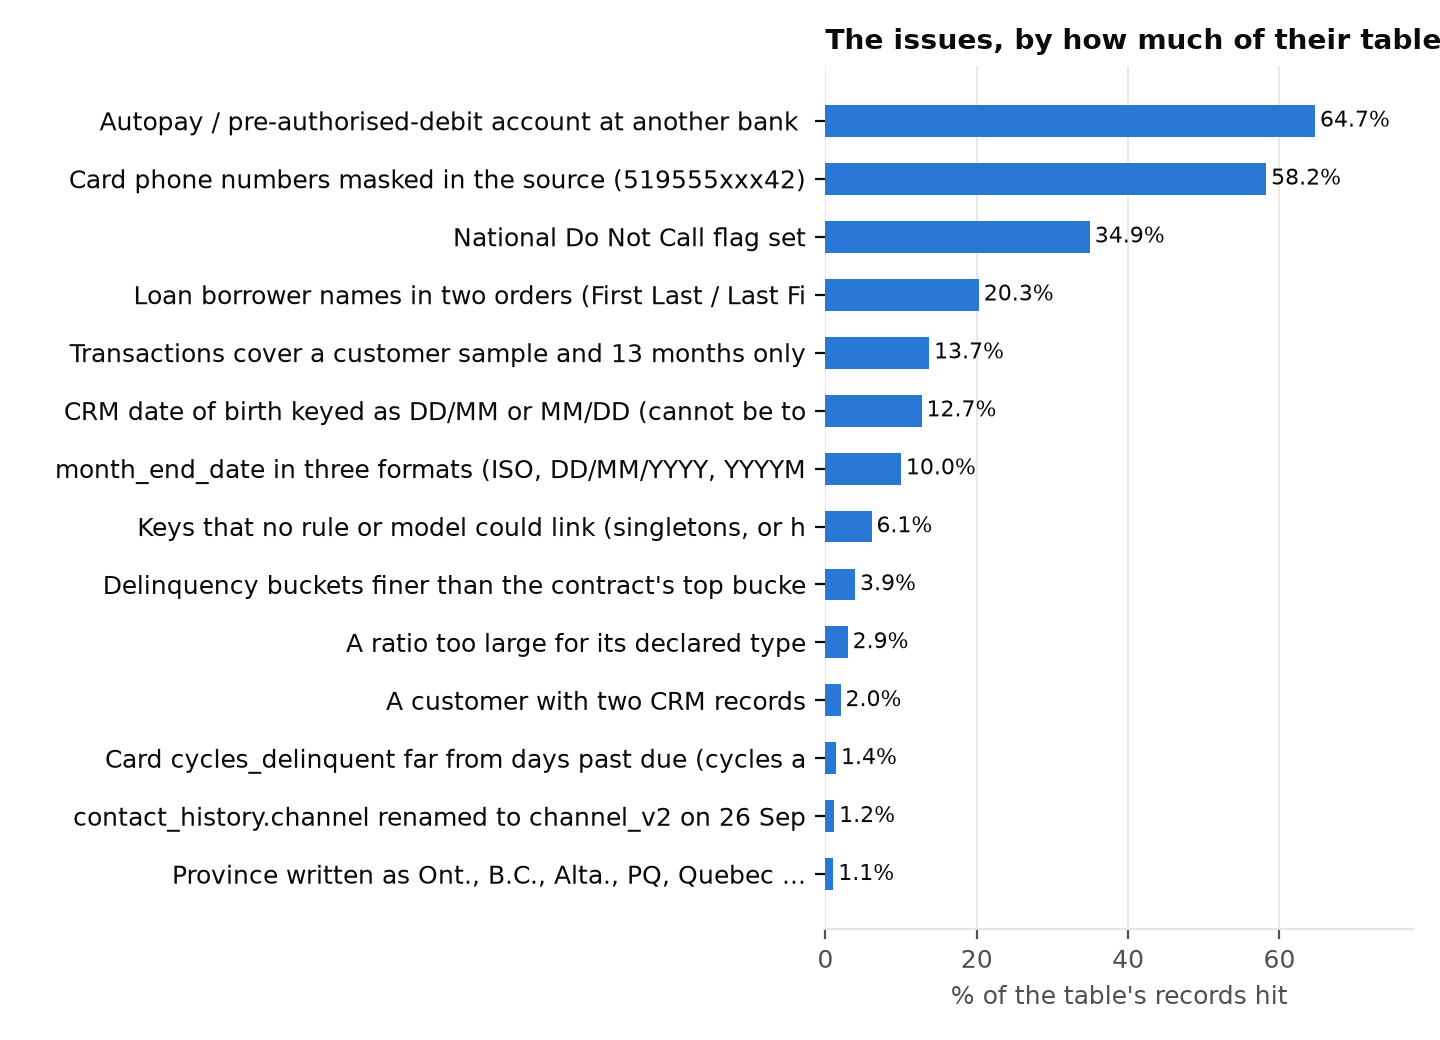
\includegraphics[width=1\linewidth,height=\textheight,keepaspectratio]{docs/reports/figures/q_issues.png}

\begin{longtable}[]{@{}
  >{\raggedright\arraybackslash}p{(\linewidth - 6\tabcolsep) * \real{0.2500}}
  >{\raggedright\arraybackslash}p{(\linewidth - 6\tabcolsep) * \real{0.2500}}
  >{\raggedright\arraybackslash}p{(\linewidth - 6\tabcolsep) * \real{0.2500}}
  >{\raggedright\arraybackslash}p{(\linewidth - 6\tabcolsep) * \real{0.2500}}@{}}
\toprule\noalign{}
\begin{minipage}[b]{\linewidth}\raggedright
Issue
\end{minipage} & \begin{minipage}[b]{\linewidth}\raggedright
Where
\end{minipage} & \begin{minipage}[b]{\linewidth}\raggedright
Records hit
\end{minipage} & \begin{minipage}[b]{\linewidth}\raggedright
Fix
\end{minipage} \\
\midrule\noalign{}
\endhead
\bottomrule\noalign{}
\endlastfoot
Agent notes with lost characters (U+FFFD) &
\texttt{agent\_notes.note\_text} & 4,636 (0.61\%) & Not recoverable: the
original characters are gone. Left as is; the redactor and extractor
read the surrounding words, which are intact. \\
CRM records deleted upstream (CDC) but still in the extract &
\texttt{customers.is\_deleted} & 2,115 (0.21\%) & Left out of silver
(the current version is deleted); listed in quarantine.customers. \\
A customer with two CRM records &
\texttt{customers\ (crm\_customer\_id)} & 20,434 (2.01\%) & Linked by
the same national ID, CRM's own duplicate pointer, or Splink (name, DOB,
phone, postal code); one golden ID each. The count is CRM records beyond
the first of each golden ID. \\
Card phone numbers masked in the source (519555xxx42) &
\texttt{card\_accounts.cardholder\_phone\_raw} & 384,422 (58.25\%) &
Cannot be normalised to a phone number: left null in the cleaned column
and listed in quarantine.card\_accounts. Cards link on name, DOB and
postal code instead. \\
CRM phone numbers cut to 9 digits &
\texttt{customers.primary\_phone\_raw} & 4,936 (0.48\%) & Not a valid
number: left null in the cleaned column, listed in
quarantine.customers. \\
CRM date of birth keyed as DD/MM or MM/DD (cannot be told apart) &
\texttt{customers.dob\_raw} & 128,980 (12.71\%) & Never guessed (reading
every slash date day-first misreads 16\% of them). CRM also holds a
clean date\_of\_birth, which is used; the raw value only fills gaps when
it is unambiguous. Cards, whose format is fixed DD-MM-YYYY, are read
day-first. \\
month\_end\_date in three formats (ISO, DD/MM/YYYY, YYYYMMDD) &
\texttt{account\_monthly\_snapshot.month\_end\_date} & 1,255,152
(9.99\%) & A plain date cast silently dropped these (1.25M values).
Silver reads all three; a month-end day is always above 12, so the DD/MM
form is unambiguous. \\
Province written as Ont., B.C., Alta., PQ, Quebec \ldots{} &
\texttt{customers.province\_code} & 10,689 (1.05\%) & Mapped to the
two-letter code (normalize\_province); gold would otherwise break the
contract. \\
A ratio too large for its declared type &
\texttt{deposit\_accounts.income\_to\_debt\_service\_ratio\_est} &
13,969 (2.94\%) & The data dictionary says decimal(8,4); values go above
9999.9999. Silver uses a wider decimal. The magnitudes look like a unit
problem upstream: not used by any feature. \\
contact\_history.channel renamed to channel\_v2 on 26 Sep &
\texttt{contact\_history.channel,\ channel\_v2} & 31,428 (1.17\%) &
Silver coalesces the two into channel (the dictionary name). \\
Loan borrower names in two orders (First Last / Last First) &
\texttt{loan\_accounts.borrower\_name\_raw} & 82,028 (20.28\%) & The
token CRM uses more as a surname is the surname
(silver.int\_name\_lexicon). Without it, loan names matched other
systems 79\% of the time; with it, 98\%. \\
Autopay / pre-authorised-debit account at another bank (not one of our
deposit accounts) &
\texttt{card\_accounts.autopay\_source\_account,\ loan\_accounts.pad\_source\_account}
& 302,549 (64.70\%) & Ignored for linking: there is nothing at our bank
to link to. Left untouched in silver. \\
National Do Not Call flag set & \texttt{customers.national\_dncl\_flag}
& 355,697 (34.94\%) & Never blocks collections contact (the list covers
telemarketing, not collections). Internal do-not-call and cease flags
do. \\
Delinquency buckets finer than the contract's top bucket (121-150,
151-180, 180+) & \texttt{collections\_cases.current\_bucket} & 14,409
(3.92\%) & Silver keeps the source label. Gold derives its bucket from
days past due, with one 121+ bucket (the shared contract). \\
Card cycles\_delinquent far from days past due (cycles are not days) &
\texttt{card\_accounts.cycles\_delinquent,\ dpd} & 673 (1.41\%) & Gold
and features use dpd, never cycles\_delinquent. \\
Contact rows whose case is not in collections\_cases (orphans; the
example contract allows \textless{} 1\%) &
\texttt{contact\_history.case\_id} & 26,864 (1.00\%) & Counted and kept
in silver; nothing joins them to a case. \\
Duplicate primary keys in the source tables &
\texttt{customers,\ contact\_history,\ promises\_to\_pay,\ agent\_notes}
& 0 (0.00\%) & None found when this report was written (the count above
is the proof). \\
Transactions cover a customer sample and 13 months only &
\texttt{transactions} & 106,914 (13.71\%) & Missing stays missing:
features from transactions are null, not 0, outside the sample. \\
Keys that no rule or model could link (singletons, or held apart) &
\texttt{gold.c360\_customer} & 64,092 (6.09\%) & Each keeps its own
golden ID with status `unlinked'. 5,498 clusters were held (two national
IDs, or more than 12 keys) and go to the steward queue. \\
\end{longtable}

\textbf{Schema drift.} \texttt{kept\ map} diffs every raw table's
columns against the data dictionary. It flags
\texttt{deposit\_accounts.overdraft\_dpd} /
\texttt{overdraft\_dpd\_bucket} (the README mentions them, the
dictionary sheet doesn't), \texttt{benchmark\_questions}, and the
transcript turn fields (they live in the JSON, not the CSV index).
\texttt{contact\_history.channel} → \texttt{channel\_v2} (renamed 26
Sep) gets merged back in silver.

\section{4. Do the tables actually
join?}\label{do-the-tables-actually-join}

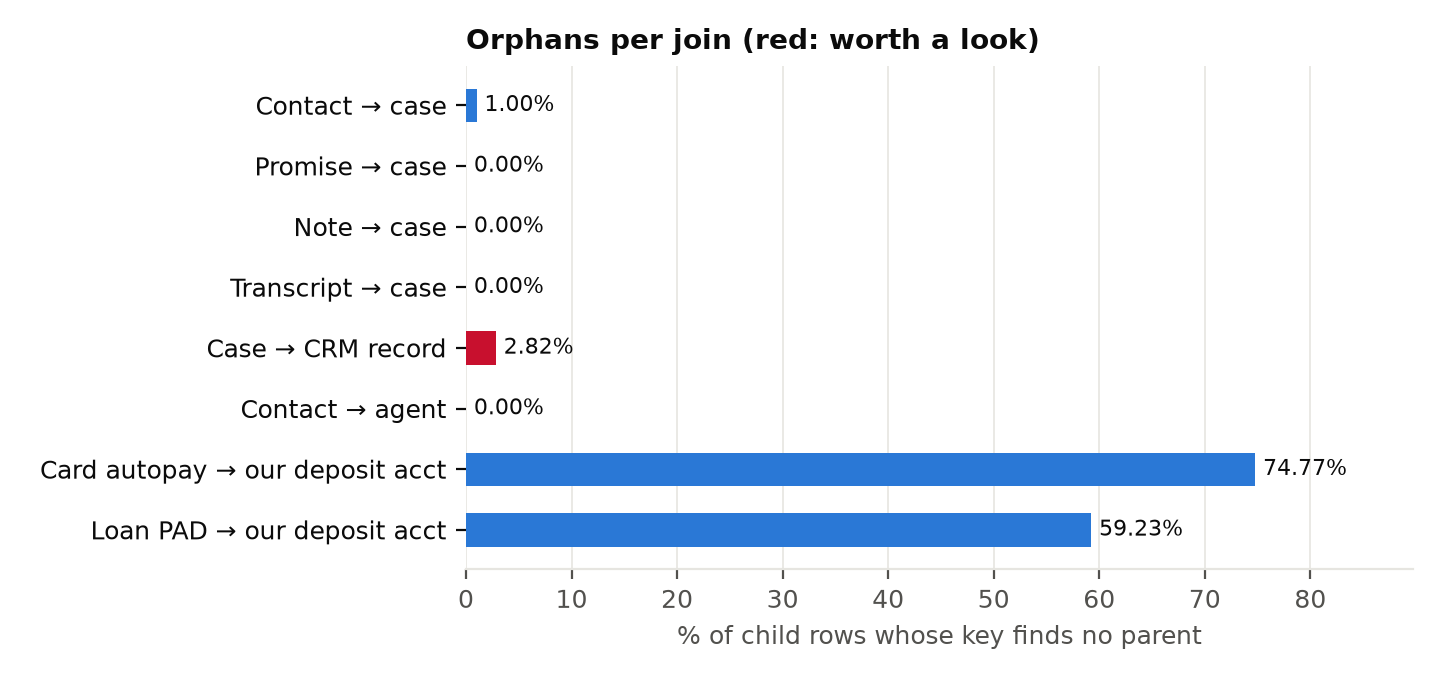
\includegraphics[width=1\linewidth,height=\textheight,keepaspectratio]{docs/reports/figures/q_links.png}

\begin{longtable}[]{@{}
  >{\raggedright\arraybackslash}p{(\linewidth - 8\tabcolsep) * \real{0.2000}}
  >{\raggedleft\arraybackslash}p{(\linewidth - 8\tabcolsep) * \real{0.2000}}
  >{\raggedleft\arraybackslash}p{(\linewidth - 8\tabcolsep) * \real{0.2000}}
  >{\raggedleft\arraybackslash}p{(\linewidth - 8\tabcolsep) * \real{0.2000}}
  >{\raggedright\arraybackslash}p{(\linewidth - 8\tabcolsep) * \real{0.2000}}@{}}
\toprule\noalign{}
\begin{minipage}[b]{\linewidth}\raggedright
Join
\end{minipage} & \begin{minipage}[b]{\linewidth}\raggedleft
Child rows with a key
\end{minipage} & \begin{minipage}[b]{\linewidth}\raggedleft
Orphans
\end{minipage} & \begin{minipage}[b]{\linewidth}\raggedleft
Share
\end{minipage} & \begin{minipage}[b]{\linewidth}\raggedright
What happens
\end{minipage} \\
\midrule\noalign{}
\endhead
\bottomrule\noalign{}
\endlastfoot
Contact → case & 2,688,337 & 26,864 & 1.00\% & kept and counted; nothing
joins them to a case \\
Promise → case & 238,815 & 0 & 0.00\% & promise features join on
case\_id \\
Note → case & 760,594 & 0 & 0.00\% & notes still feed hardship by
customer \\
Transcript → case & 25,000 & 0 & 0.00\% & call summaries look calls up
by case \\
Case → CRM record & 367,229 & 10,365 & 2.82\% & other exact rules +
Splink still resolve them; every open case resolves (gate Q2) \\
Contact → agent & 1,018,776 & 0 & 0.00\% & blank for automated
contacts \\
Card autopay → our deposit acct & 164,565 & 123,047 & 74.77\% & account
at another bank: ignored for matching \\
Loan PAD → our deposit acct & 303,037 & 179,502 & 59.23\% & same \\
\end{longtable}

The one worth flagging: \textbf{10,365 cases (2.82\%) point at a CRM ID
that isn't in \texttt{customers}.} They're not lost: card, loan and
deposit keys plus Splink still put them on a person, and the gate checks
that every \emph{open} case resolves. The autopay/PAD numbers are high
on purpose: most of those accounts are at other banks, so we never use
them to link anyone.

\section{5. Identity resolution (the bit that can actually hurt
someone)}\label{identity-resolution-the-bit-that-can-actually-hurt-someone}

There's no shared customer ID across the five systems. We link in two
passes:

\begin{enumerate}
\def\labelenumi{\arabic{enumi}.}
\tightlist
\item
  \textbf{Exact rules}: keys we can prove (the case's copy of the CRM
  ID, autopay/PAD → our deposit account, the same national ID hash,
  CRM's own duplicate pointer, and the core-banking customer number
  shared by deposits and the bureau file).
\item
  \textbf{Splink} (Fellegi--Sunter) on what's left, comparing name, date
  of birth, phone and postal code. \textbf{≥ 0.95 links automatically,
  0.80--0.95 goes to a data steward, lower stays apart.} A cluster with
  two national IDs or more than 12 keys is never auto-merged.
\end{enumerate}

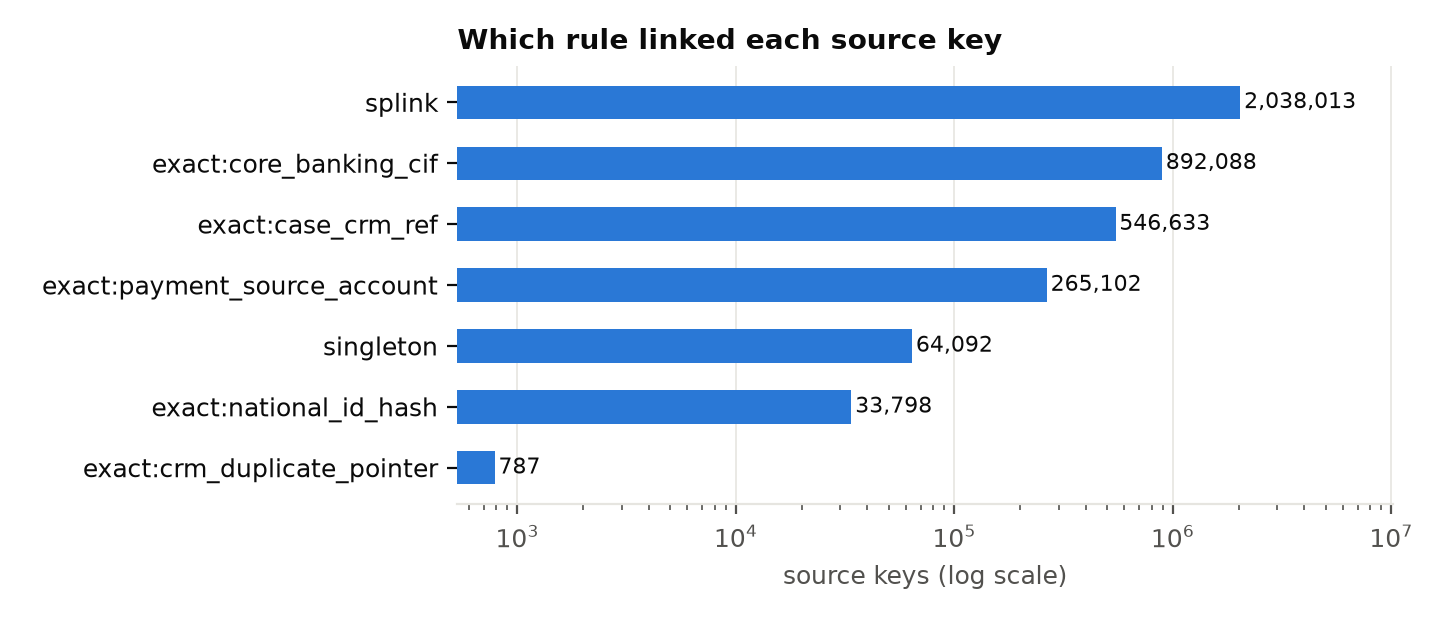
\includegraphics[width=1\linewidth,height=\textheight,keepaspectratio]{docs/reports/figures/q_rules.png}

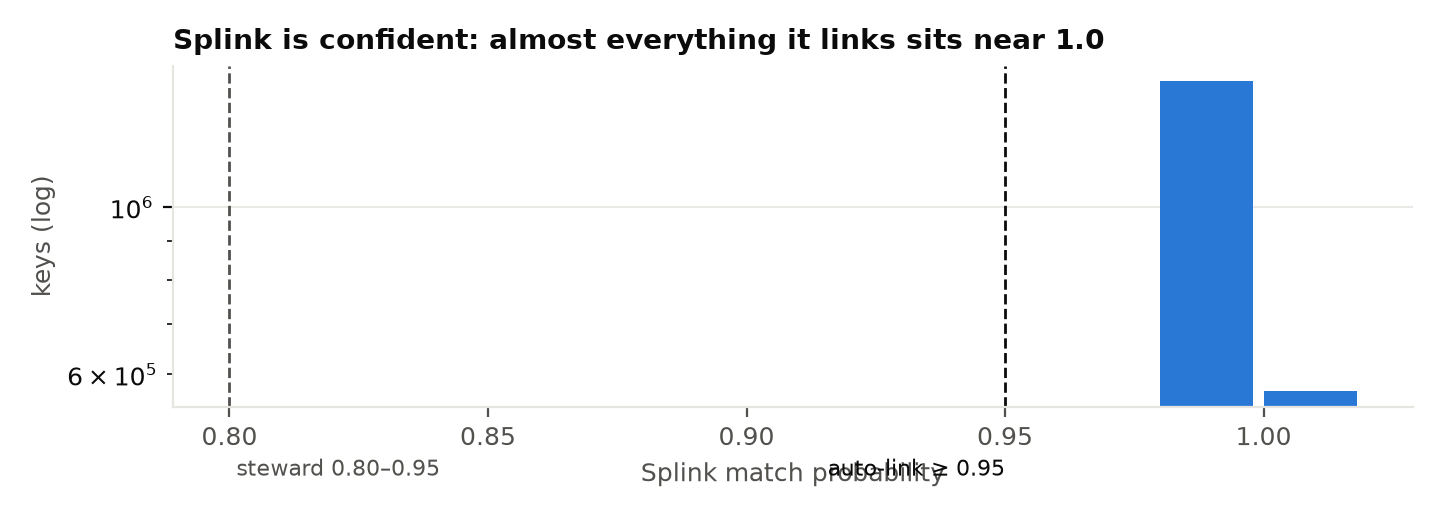
\includegraphics[width=1\linewidth,height=\textheight,keepaspectratio]{docs/reports/figures/q_scores.png}

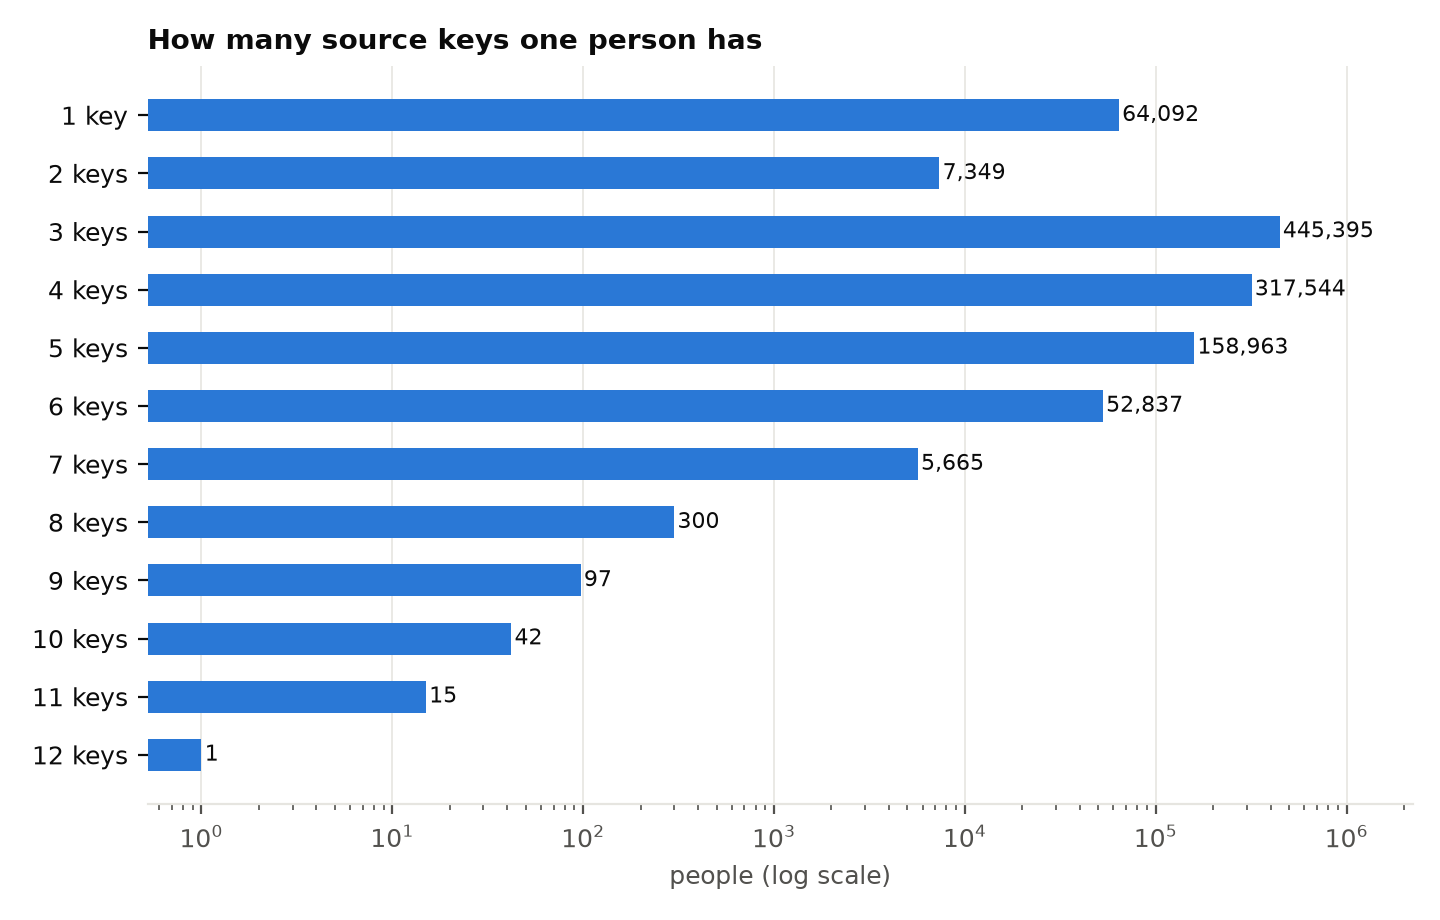
\includegraphics[width=1\linewidth,height=\textheight,keepaspectratio]{docs/reports/figures/q_sizes.png}

\textbf{The human check.} No ground-truth IDs came with the data, so a
person reviewed 300 random predicted links, sorted into tiers by how
many identifiers agree (tier 1: 276, tier 2: 14, tier 3: 10).

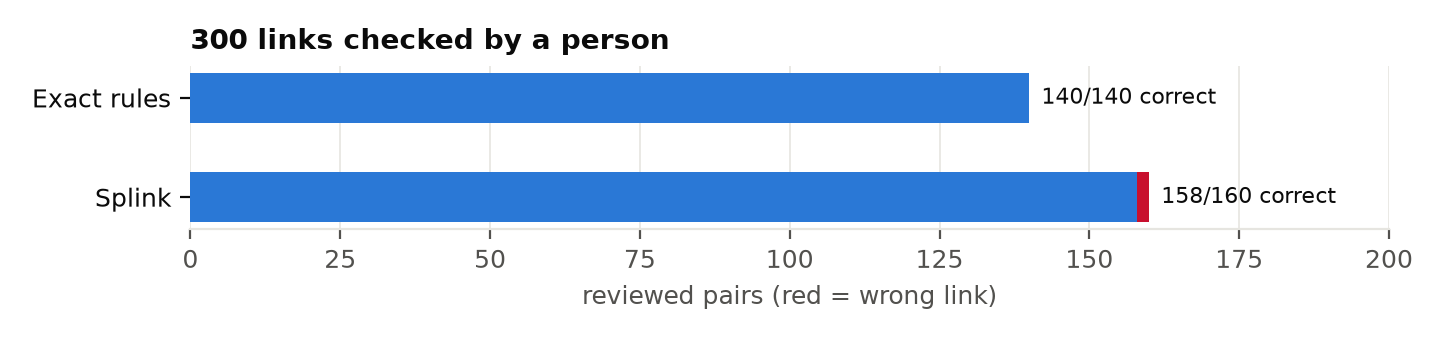
\includegraphics[width=1\linewidth,height=\textheight,keepaspectratio]{docs/reports/figures/q_review.png}

Both wrong links (MP-238, MP-239) are Splink pairs where everything
matched except the surname, and both scored 1, 1. A stricter threshold
wouldn't have caught them; the human did. That's why the review sample
stays in the pipeline.

Golden IDs are stable run to run (last run: 0 merged, 0 split). The
golden record has 1,052,300 people: 64,092 are single keys nothing could
link, 37,042 carry \texttt{do\_not\_contact} and 23,593
\texttt{collections\_hold}, each set if \textbf{any} linked record says
so. Hardship status: none 991,933, confirmed 32,306, possible 28,061.

\section{6. The contract gate}\label{the-contract-gate}

\texttt{contracts/c360\_customer.odcs.yaml} is built from the
organisers' example DC-COLL-001 (owner, refresh, quality rules, allowed
and not-allowed uses) and extended to ODCS v1.0.0. Publishing is blocked
unless:

\begin{longtable}[]{@{}
  >{\raggedright\arraybackslash}p{(\linewidth - 4\tabcolsep) * \real{0.3333}}
  >{\raggedright\arraybackslash}p{(\linewidth - 4\tabcolsep) * \real{0.3333}}
  >{\raggedright\arraybackslash}p{(\linewidth - 4\tabcolsep) * \real{0.3333}}@{}}
\toprule\noalign{}
\begin{minipage}[b]{\linewidth}\raggedright
Rule
\end{minipage} & \begin{minipage}[b]{\linewidth}\raggedright
Status
\end{minipage} & \begin{minipage}[b]{\linewidth}\raggedright
Detail
\end{minipage} \\
\midrule\noalign{}
\endhead
\bottomrule\noalign{}
\endlastfoot
Q1-unique-ids & \textbf{PASS} & 1,052,300 golden IDs unique; every
active source key maps to one \\
Q2-linkage & \textbf{PASS} & 98.66\% of account keys linked; every open
case resolves \\
Q3-match-safety & \textbf{PASS} & every auto link scores \textgreater=
0.95; no cluster holds two national IDs \\
Q3-review-precision & \textbf{PASS} & precision 99.3\% on 300 reviewed
predicted links; 300 of 300 pairs reviewed \\
Q4-contact-safety & \textbf{PASS} & 0 violations \\
Q5-freshness & \textbf{PASS} & published 0.1h after the source
extract \\
Q5-row-count & \textbf{PASS} & 1,052,300 rows, +0.0\% vs the last
load \\
hardship-text & \textbf{PASS} & 785,594 extractions; 11,464 golden IDs
rest on them \\
\end{longtable}

\section{7. Text, features, monitoring}\label{text-features-monitoring}

\begin{itemize}
\tightlist
\item
  \textbf{Redaction first, always.} All 760,594 notes and 25,000
  transcripts go through Presidio (English + French spaCy, Canadian SIN
  and postal codes, mangled cards and dates of birth). Full scan after:
  \textbf{0} leftovers. The LLM gateway won't even accept un-redacted
  text.
\item
  \textbf{Labels: public only.} Text models are tuned and tested on the
  release's 500 public labels per source (30\% held out). The rest are
  the organisers'.
\item
  \textbf{Parity:} PASS: 0 of 56,000 cells differ (0.0000\%; the limit
  is 0.1\%).
\item
  \textbf{Drift:} 10 features drift, 5 to watch, 11 stable (PSI vs
  training); 3 payroll features never appear in training rows.
\item
  \textbf{Missing stays missing.} Transactions only cover a sample of
  customers and 13 months; outside that, those features are null, not 0.
\end{itemize}

\section{8. What we can't measure}\label{what-we-cant-measure}

\begin{itemize}
\tightlist
\item
  \textbf{True match accuracy.} No ground truth; §5's human review and
  the exact-rule cross-check are the evidence.
\item
  \textbf{Monthly roll rates.} The account snapshot only has
  quarter-ends (Dec 2023--Jun 2026), so roll rates are quarterly.
\item
  \textbf{Generation rules.} The README says some fields were set by
  rule; we take them as given.
\end{itemize}

\section{9. If we owned the source
systems}\label{if-we-owned-the-source-systems}

\begin{enumerate}
\def\labelenumi{\arabic{enumi}.}
\tightlist
\item
  Put one customer ID (or the CIF) in CRM: 892,088 of our links lean on
  a number only deposits and the bureau carry.
\item
  One date-of-birth format on the entry screen: 12.7\% of CRM DOBs are
  ambiguous today.
\item
  Stop masking card phone numbers in the extract (58\% are useless for
  matching).
\item
  Ship schema changes (\texttt{channel\_v2}, the overdraft columns) in
  the dictionary first.
\item
  Keep a 300-link human review per release; it caught the only two bad
  links.
\end{enumerate}

\emph{Rebuild:}
\texttt{uv\ run\ kept\ gate\ \&\&\ uv\ run\ python\ scripts/quality\_report\_full.py}
(with \texttt{kept\ serve} stopped).

\end{document}
